\documentclass[12pt,answers]{exam}
\usepackage{amsmath,amsfonts,amssymb,commath,mathtools,physics}
\usepackage{todonotes}
\usepackage{enumitem}
\usepackage{float}
\newcommand{\vect}[1]{\left\langle #1 \right\rangle}
\newcommand{\tcurl}{\operatorname{curl}}
\newcommand{\tdiv}{\operatorname{div}}
\newcommand{\tgrad}{\operatorname{grad}}
\newcommand{\RR}{\mathbb{R}}

\pagestyle{headandfoot}
\firstpageheadrule
\runningheadrule
\firstpageheader{Math 222}{Final Exam Version A|Solutions, Page \thepage\ of \numpages}{December 12, 2018}
\runningheader{Math 222}{Final Exam Version A|Solutions, Page \thepage\ of \numpages}{December 12, 2018}
\runningfooter{}{}{}

\title{2018 Fall Calc 3 Final Version A|Solutions}
\author{Winston Cheong}
\date{}

\begin{document}
% \maketitle
\begin{questions}
	\question Here is a vector which you can assume has unit length:
	\begin{figure}[H]
		\centering
		\vspace{.5in}
		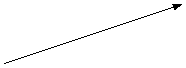
\includegraphics{graphics/2018-fall-final-va-1.pdf}
		\vspace{.5in}
	\end{figure}
	Call this vector $\vb{u}$. Now using the same base point draw a vector $\vb{w}$ (and label it) so that the following are all satisfied:
	\begin{enumerate}[label=(\alph*)]
		\item $|\vb{w}| = 1$.
		\item $\vb{u} \cross \vb{w}$ points away from you
		\item $\vb{u} \cross \vb{w} \approx \sqrt 2/2$. (Try to make it as close as you can.)
	\end{enumerate}
	Next using the same base point again draw a vector $\vb{v}$ (and label it) so that the following are all satisfied:
	\begin{enumerate}[label=(\alph*)]
		\item $|\vb{v}| = 1$.
		\item $\vb{u} \vdot \vb{v} \approx 1/2$. (Again, do your best to get equality.)
		\item $\vb{u} \cross \vb v$ points toward you.
	\end{enumerate}
	\begin{solution}
		\begin{align*}
			\vb u \cross \vb w &= \| \vb u \| \|\vb w\| \sin \theta = \sqrt 2/2 \implies \theta = 45^\circ \\ 
			\vb u \vdot \vb v &= \| \vb u \| \|\vb v\| \cos \theta =  1/2 \implies \theta = 60^\circ
		\end{align*}
		so the final configuration looks like
		\begin{figure}[H]
			\centering
			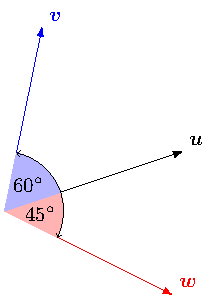
\includegraphics{graphics/2018-fall-final-va-1-sol.pdf}
		\end{figure}
	\end{solution}

	\newpage
	\question
	Short answers\ldots Intuition and Understanding
	\begin{parts}
		\part If you are driving, then what device (or devices) in your car will be the best way to change your normal acceleration?
		\begin{solution}
			Steering wheel
		\end{solution}

		\part What is the curvature of a circle with radius 81?
		\begin{solution}
			$\kappa = \frac{1}{81}$
		\end{solution}

		\part $f(x,y)$ is defined to equal 2 for all points on the disk $(x-1)^2 + (y-2)^2 \le 9$, to equal $-3$ for all points on the disk $(x+4)^2 + (y+7)^2 \le 4$, and to equal 0 everywhere else. Compute:
		\[
			\int_{x=-90}^{100} \int_{y=-100}^{90} f(x,y) \dif y \dif x.
		\]
		\begin{solution}
			$= 2 \cdot \pi (3^2) + -3 \pi (2^2) = \boxed{6\pi}$
		\end{solution}

		\part Will the surface integral
		\[
			\iint_{S} f(x,y,z) \dif S
		\]
		typically give you the surface area of $S$? Explain your answer in one sentence or less.
		\begin{solution}
			No. Only if $f(x,y,z) = 1$ will the integral compute the surface area of $S$.
		\end{solution}
		\part What is the average value of the function $f(x,y) = 3 + 2y$ on the rectangle $1\le x \le 5$, $2 \le y \le 4$?
		\begin{solution}
			\[
				= \frac{\int_1^5 \int_2^4 3+2y \dif y \dif x}{(5-1)(4-2)} = \frac{4 [3y + y^2]_2^4}{2\cdot 4} = \boxed{9}
			\]
		\end{solution}
	\end{parts}

	\newpage
	\question
	Short answers\dots Definitions and Theorems
	\begin{parts}
		\part Suppose that $\nabla f(0,0) = \vect{0,0}$, and $f_{xx}(0,0)$ and $f_{yy}(0,0)$ are both negative. Do you need anything else to conclude that $(0,0)$ is a local maximum? (If yes, then what? If no, then why not?)
		\begin{solution}
			Yes, need to know that the discriminant $> 0$.
			In particular, that $f_{xx}(0,0) f_{yy}(0,0) > f_{x,y}(0,0)^2$.
		\end{solution}
		\part What does it mean (definition!) for a vector field $\vb{F}(x,y,z)$ to be incompressible?
		\begin{solution}
			$\tdiv \vb{F} = 0$.
		\end{solution}
		\part According to the theorem that we learned, if $f$ is a continuous function on a set $\Omega$, then what condition or conditions on $\Omega$ will guarantee that $f$ attains an absolute maximum and absolute minimum?
		\begin{solution}
			$\Omega$ must be closed and bounded
		\end{solution}
		\part Assume that you have been given a differentiable vector field defined on the first octant. How can you quickly tell if it is conservative?
		\begin{solution}
			If it is conservative, one should produce a potential function.
			If it is not conservative, one should show it violates the cross partials property.
		\end{solution}
	\end{parts}

	\newpage 
	\question
	A certain differentiable function satisfies:
	\begin{enumerate}[label=(\alph*)]
		\item $f(7, -9) = 1$, and $f(-2, 4)= 6$
		\item $\nabla f(7, -9) = (5,3)$, and $\nabla f = (-2, 4) = (8, -\pi)$.
	\end{enumerate}
	At each of the two points in question (i.e.~at $(7, -9)$ and at $(-2 ,4)$) answer the following questions:
	\begin{parts}
		\part In what direction is the function increasing the fastest?
		\begin{solution}
			For $(7, -9)$: $\vect{5, 3}$; 
			For $(-2, 4)$: $\vect{8, -\pi}$.
		\end{solution}

		\part What is the rate of change in that direction?
		\begin{solution}
			For $(7, -9)$: $\sqrt{25 + 9} = \sqrt{34}$;
			For $(-2, 4)$: $\sqrt{64+\pi^2}$.
		\end{solution}

		\part What is the directional derivative in the direction of $\vect{3,-4}$? (Note: just to be completely clear about semantics here, you are supposed to give the same directional derivative at each point. I did not ask for the directional derivative in the direction of the point $(3, -4)$.)
		\begin{solution}
			Let $\vb u = \vect{\frac35, -\frac45}$.

			For $(7, -9)$: $D_{\vb u} f(7, -9) = \nabla f(7, -9) \vdot \vb{u} = \vect{5,3} \vdot \vect{\frac35, -\frac45} = \frac35$. \\ 
			For $(-2, 4)$: $D_{\vb u} f(-2, 4) = \nabla f(-2, 4) \vdot \vb{u} = \vect{8, -\pi} \vdot \vect{\frac35, -\frac45} = \frac{24+4\pi}{5}$.
		\end{solution}

		\part What is the tangent plane and/or the linear approximation at each of the two points?
		\begin{solution}
			For $(7, -9)$: $L(x, y) = 1 + 5(x-7) + 3(y+ 9)$\\
			For $(-2, 4)$: $L(x, y) = 6 + 8(x+2) - \pi(y - 4)$
		\end{solution}
	\end{parts}

	\newpage
	\question
	Find the maximum and minimum of the function
	\[
		f(x,y) = 4x^2 - x + 4y^2 - 2y
	\]
	on the set 
	\[
		g(x,y) = x^2 + y^2 \le 45.
	\]
	Show your work carefully, and explain what you are doing. (No essays, please. Just a few short words in the right places will suffice.)
	\begin{solution}
		First, consider $g < 45$. Setting $\nabla f = 0$, and solving
		\[
			\nabla f = \vect{8x-1, 8y-2} = \vb 0
		\]
		gives the critical point $(\frac18, \frac14)$.
		Next, considering $g = 45$, we solve $\nabla f = \lambda \nabla g$:
		\[
			\left\{
				\begin{aligned}
					8x-1 &= 2\lambda x \\ 
					8y-2 &= 2\lambda y\\
					x^2 + y^2 &= 45
				\end{aligned}
			\right.
		\]
		The first two equations give
		\[
			x = \frac{1}{8-2\lambda}\qquad y = \frac{2}{8-2\lambda}
		\]
		Substituting into the the third equation gives
		\[
			\frac{5}{(8-2\lambda)^2} = 45 \implies \frac{1}{(8-2\lambda)^2} = 9 \implies \frac{1}{8-2\lambda} = \pm 3
		\]
		which yields the two constrained critical points: $(3, 6)$, $(-3, -6)$.
		Evaluating $f$ on the found critical points:
		\begin{align*}
			f(\frac18, \frac14) &= -\frac{5}{16} \\ 
			f(3, 6) &= 165 \\ 
			f(-3, -6) &= 195
		\end{align*}
		Thus the maximum is 195, and the minimum is $-\frac{5}{16}$.
	\end{solution}

	\newpage
	\question
	Let $S$ be the part of the set 
	\[
		z = x^2 + y^2
	\]
	which is between the planes $z=4$ and $z=9$. \\ 
	Express the surface area for $S$ as an iterated integral (i.e.~a double or triple integral) over a subset of $\RR^2$ or $\RR^3$ which has \textbf{constant} bounds of integration. (i.e.~it should be over a rectangular solid or a rectangle in the domain in which you are finally integrating.) You do \textbf{NOT} need to find this integral.
	\begin{solution}
		The set $S$ can be parametrized by 
		\[
			G(r, \theta) = (r\cos \theta, r\sin\theta, r^2) \qquad 2 \le r \le 3, \ 0 \le \theta \le 2\pi
		\]
		We can then compute
		\begin{align*}
			\vb{N} = G_r \cross G_\theta 
			&= \vect{\cos \theta, \sin\theta, 2r} \cross \vect{-r\sin\theta, r\cos\theta, 0}  \\ 
			&= \vect{-2r^2\cos\theta, -2r^2\sin\theta, r}
		\end{align*}
		and
		\[
			\|\vb{N}\| = \sqrt{4r^4+r^2}
		\]
		The surface area of $S$ can thus be computed as the surface integral
		\[
			\iint_S 1 \dif S  = \boxed{\int_0^{2\pi} \int_2^3 \sqrt{4r^4+r^2} \dif r \dif \theta}
		\]
	\end{solution}

	\newpage
	\question
	Let $C$ be the curve given by 
	\[
		\vb{r}(t) = \left(t \cdot \cos(5\pi t), t + \sin(5\pi t), \frac{t^3}{4+t^2}\right), 
	\]
	with $0 \le t \le 2$. Compute the following integral: 
	\[
		\int_C \vect{z, 3y^2, x} \vdot \dif \vb{r}.
	\]
	\begin{solution}
		Note that the vector field $\vb{F} = \vect{z, 3y^2, x}$ is conservative, with potential function $f = xz + y^3$.
		Hence this line integral can be computed as
		\begin{align*}
			\int_C \vect{z, 3y^2, x} \vdot \dif \vb{r}
			&= f(\vb{r}(2)) - f(\vb{r}(0)) \\ 
			&= f(2,2,1) - f(0,0,0) \\ 
			&= 10 - 0 = \boxed{10}
		\end{align*}
	\end{solution}

	\newpage
	\question
	Let $Q$ be the set of points within the set:
	\[
		\{ (x,y,z) : x^2+y^2+z^2 \le 4, \quad \text{and } 0 \le x \}
	\]
	and let $\partial Q$ be the boundary of this set. If $\vb{n}$ is the outward unit normal to this region, then compute:
	\[
		\iint_{\partial Q} (x^2, \cos(z^4), \sin(y^4)) \vdot \vb{n} \dif S.
	\]
	\begin{solution}
		By the divergence theorem, 
		\[
			\iint_{\partial Q} \vb{F} \vdot \dif \vb{S} = \iiint_{Q} \tdiv \vb F \dif V
		\]
		so 
		\begin{align*}
			\iint_{\partial Q} (x^2, \cos(z^4), \sin(y^4)) \vdot \vb{n} \dif S
			&= \iiint_Q 2x \dif V
		\end{align*}
		Evaluating this integral in spherical coordinates,
		\begin{align*}
			\iiint_{Q} 2x \dif V 
			&= \int_{-\pi/2}^{\pi/2} \int_0^\pi \int_0^2 2 \rho \sin\varphi \cos\theta \cdot \rho^2 \sin\varphi \dif \rho \dif \varphi \dif \theta\\
			&= \int_0^2 2\rho^3 \dif \rho \cdot \int_0^\pi \sin^2\varphi \dif \varphi \cdot \int_{-\pi/2}^{\pi/2} \cos\theta \dif \theta\\
			&= \left[ \frac{\rho^4}{2} \right]_0^2 \cdot \int_0^\pi \frac12 - \frac12 \cos 2\varphi \dif \varphi \cdot \left[\sin\theta\right]_{-\pi/2}^{\pi/2} \\ 
			&= 8 \cdot \left[ \frac12 \varphi - \frac14 \sin 2\varphi\right]_0^\pi \cdot 2 \\ 
			&= \boxed{8\pi}
		\end{align*}
	\end{solution}

	\newpage
	\question
	Let $E$ be the subset of
	\[
		z = x^2 + y^2
	\]
	which also satisfies 
	\[
		z \le 25, \qquad x \le 0, \qand y \ge 0.
	\]
	Express
	\[
		\iint_E x^2 \dif S
	\]
	as an iterated integral (i.e.~a double or triple integral) over a subset of $\RR^2$ or $\RR^3$. You do \textbf{NOT} need to find this integral.
	\begin{solution}
		The set $E$ can be parametrized by 
		\[
			G(r, \theta) = (r \cos \theta, r\sin\theta, r^2) \qquad 0 \le r \le 5, \ \frac\pi2\le \theta\le \pi
		\]
		Then we can compute
		\begin{align*}
			\vb{N} = G_r \cross G_\theta 
			&= \vect{\cos \theta, \sin\theta, 2r} \cross \vect{-r\sin\theta, r\cos\theta, 0}  \\ 
			&= \vect{-2r^2\cos\theta, -2r^2\sin\theta, r}
		\end{align*}
		and
		\[
			\|\vb{N}\| = \sqrt{4r^4+r^2}
		\]
		Which allows to rewrite the integral as
		\[
			\iint_E x^2 \dif S = \boxed{\int_{\pi/2}^\pi \int_0^5 r^2 \cos^2\theta \cdot \sqrt{4r^4+r^2} \dif r \dif \theta}
		\]
		
	\end{solution}

	\newpage
	\question
	Let $E$ be the part of the set
	\[
		\sqrt{x^2+y^2} \le z \le 5
	\]
	that also satisfies
	\[
		y \le 0.
	\]
	Find 
	\[
		\iiint_{E} y \dif V.
	\]
	\begin{solution}
		$E$ is half of a solid cone.
		The integral can be written in cylindrical coordinates as
		\begin{align*}
			\int_0^5 \int_r^5 \int_\pi^{2\pi} r \sin\theta \cdot r \dif \theta \dif z \dif r
			&= \int_0^5 \int_r^5 r^2 \dif z \dif r \cdot \int_\pi^{2\pi} \sin\theta\dif \theta \\ 
			&= \int_0^5 r^2 (5-r) \dif r \cdot [-\cos \theta]_\pi^{2\pi} \\
		&= \left[\frac53 r^3 - \frac14 r^4 \right]_0^5 \cdot -2 \\
		&= 5^4 \left(\frac13 - \frac 14\right) \cdot -2 = \boxed{-\frac{5^4}{6}}
		\end{align*}
	\end{solution}

\end{questions}

\end{document}
